
\section{Process Background}
    Discussion of Form Factors and genralized proton structure, Wigner Functions

PAGE 245 OF FNPP FOR GDP STUFF
        FNPP GPD discussion on page 232
        
    Now discussion of DVEP:
GPDs, Wigner functions
relationships all the way around
some annoying math
Handbag diagram
Lepton hadron plane
Status of experiments and future (EIC mapping)

        As we increase the resolution (resolve features over smaller spatial distances), what we see is dependent on what resolution scale we are at. An exception to this case is if we are investigating point-like particles, which would have an identical response across all resolution scales


Deep exclusive processes can allow access to Generalized Parton Distributions (GPDs),
a concept that lies at the root of 3D imaging of the proton’s quark-gluon substructure,
as GPDs contain information about the transverse spatial distribution of quarks and their
longitudinal momentum inside hadrons. The key to extracting GPDs from experiments are
the Quantum Chromodynamics (QCD) factorization theorems. Deeply Virtual Compton
Scattering (DVCS) is the cleanest way to
study GPDs. While DVCS data have given hints of the factorization regime being
attained, such hints have not been observed for Deeply Virtual Meson Production (DVMP)
data. Exclusive $\pi^0$ electroproduction has been measured by experiment E12-06-114 in Hall
A of JLab in order to test factorization in DVMP processes. Cross sections have been
measured at three fixed Bjorken- x (xB) : 0.36, 0.48 and 0.6 in the Q2 range 3 to 9 GeV2.
High statistical measurements of polarized and unpolarized cross sections of H(e,e’,gamms)
p could allow mapping and extraction of GPD information from the nucleon. In this talk,
I will show the experimental setup, calibration and preliminary results of the neutral pion
electroproduction cross sections for xB 0.3 from this experiment


Intuition about DVMP
First, note that not all DVMP reactions are sensitive to nuclear transversity distributions,
which involves quark helicity flip of transversely polarized quarks helicity This can occur
in production of pseudoscaler mesons, e.g. pi0 and eta production, with spin-charge-parity
I-PC= 0 - + ,in contrast with the incident photon, which has J-P 1- -. This is not the case
for other mesons studied at JLab, such as vector mesons, I-PC= 0 - e.g. the rho, omega, phi,
for which which I-CP= 1- -, the same as for the photons. I believe this was first pointed out
Ahmad, Goldstein, Liutti (arXiv:0805.3568). Here is a quote from their intro. ”... deeply
virtual $\pi^0$ (as well as$\eta$,$\eta$') production off a proton target is clearly distinct from the other
types of meson production processes in that it involves the transition of a (virtual) photon
with JPC = 1– to a JPC = 0-+ state (i.e. the final $\pi^0$ or$\eta$,$\eta$’) requiring odd C-parity and
chiral odd t-channel quantum numbers. As a consequence, in a partonic description such
as the one depicted in Fig.1a, the ”outgoing” and ”returning” quark helicities need to be
opposite to one another . . . ”.
Peter Kroll, who works very closely this group, with Sergei Goloskokov, Marcus Diehl,
et al. have published extensive theoretical calculations based on Jlab data. Gary Goldstein,
Simonetta Liutti have have also published on this reaction.
By the way, the other meson production channels are uniquely sensitive to other inter-
esting aspects of nucleon structure. For example, the phi, on which F-X and Patrick are
working, is very sensitive to the gluon distribution in the nucleon.
In DVCS the incident and outgoing particles are both photons JP= 1-. Therefore, no
quark helicity flip is necessary in this “virtual Compton scattering”. Therefore DVCS is
primarily sensitive to non-quark spin flip - eg. H.. The same is true with DVMP of other
vector meson, such as rho. However, since the pi0 and eta are JP=0-, then the transverse
photon part contributing to the overall reaction cross section can cause a transversely po-
larized quark helicity flip. This is contained mainly in the structure functions $\sigma$T and $\sigma$T T ,
which can be decomposed into the transverity GPDs - mainly EbarT and HT

Also, pion and eta production can still also be accompanied by non-quark helicity flips,
which would be mainly contained in the longitudinal structure functions $\sigma$LL. However,
various theoretical papers indicate that in our accessible region of Q2, $\sigma$T and $\sigma$T T dominate
relative to $\sigma$L. Experimentally, this seems to be verified from JLab data . On the other
hand, theory predicts that asymptotically, $\sigma$L will dominate. From our existing 5 GeV data,
we are not anywhere near there, so our experiments at JLab are really just right for accessing
these transversity distributions. But, to decompose these distributions at the level of the
individual quark u d flavors, we need as much precision data over as big a range as possible
of kinematics in several channels - P-pi0, N-pi0, P-eta, N-eta. And, only you guys can do
that! So, let me know if this makes sense to you. s a bit.

What do we want at the end of the day and why?
What is the Hall A DVMP measurement? gravitational form factor of the proton Why is
CLAS12 particularly suited for this measurement Compare to other experiemnts - hall A,
compass, etc. Precision estimate – 10\%? 5\% if we are lucky? What was precision of CLAS6?
other note – intution for process – not just getting longitudinal momentum information as
with DIS, but also get the other piece of information from having put back together the
proton. Read about Compton Form Factors/ extensions of. of all electrons that enter target,
how many colissions do we get? probably either 1 or none? what is the probability of 1?
Very important and good stating place - write up notes from 2011 pi0 analysis note
Write to Axel at BIn Volume correction, page 75 analysis note fig 6.1
Compare integrated luminosity of CLAS6 to CLAS12 (in 2011 analysis note)
$\pi^0$ $\rightarrow$ $\gamma$$\gamma$ branching ratio = 98.8\%
Given we have an interaction, how many do we detect (ep)?
Question: WHy is beam charge important? Answer (Brandon Clary, email) The accu-
mulated beam charge is charge measured at the Faraday cup. It’s important for determining
the luminosity for a run, and even being able to compare data from run to run, especially
when runs may have different beam current, for example. It’s just a good way to normalize
to the total number of electron in that run, file, etc. In principle you could normalize by
minutes, hours, etc. But beam charge, number of el., is needed to calculate the luminosity
for a fixed target experiment when extracting cross sections.
263

Low t-data are very important for the meson exclusive physics. The GPD interpretation
works only in the region -t/Q2¡1. From this point of view the central detector will not only
increase the total statistics by a factor more than 2 but will add the valuable data with low
t.
However, for pi0 the only data we have from Hall A are of very limited statistics and
kinematics. One of their limitations was the relatively modest variation on polarization
parameter (epsilon) since the beam energies we not so far apart.
Number of final events in CLAS6 DVMP? About 100K, maybe 200K.
Dear Valery
CLAS12 acceptances and resolutions are also superior to that of CLAS6. Main differences
are: - RGK has outbending torus vs inbending CLAS6 data - the distance between the target
and the PCal has increased, the FTCal extends to lower angles, and the gap between FTCal
and PCal is much smaller than between IC and EC - proton polar angle was limited to 60
deg in the e1dvcs dataset if my memory is correct
Do you have on hands the number of exclusive pi0 events published for the CLAS6
cross-sections? We need numbers to make the case to cook the RGK data
Well over an order of magnitude more statistics at CLAS12 compared to CLAS6


invariant mass is W 

GPDs combine the kinematics of both elastic form factors and parton distributions. Andrey references 5, 6, and 7


\subsection{Generalized Parton Distributions}

          The cross-section for DV$\pi^0$P \eqref{DVPiPCrossSection_theory} can be theoretically linked in terms of structure functions to GPDs, which describe the 3D structure of the nucleon.


          
    
     \begin{equation}\labelAndRemember{eq:DVPiPCrossSection_theory}
           {\frac{d^4\sigma_{\gamma^*p \rightarrow p'\pi^0}}{dQ^2dx_Bdtd\phi_{\pi}} =
         \Gamma (Q^2, x_B, E)
         \frac{1}{2\pi}
         \left\{ \left(  \textcolor{sigmaT}{\frac{d\sigma_T}{dt}}+\epsilon  \textcolor{sigmaL}{\frac{d\sigma_L}{dt}} \right)+
         \epsilon cos(2\phi)  \textcolor{sigmaTT}{\frac{d\sigma_{TT}}{dt}} + 
         \sqrt{2\epsilon(1+\epsilon)} cos(\phi)  \textcolor{sigmaLT}{\frac{d\sigma_{LT}}{dt}} \right\}}
     \end{equation}      \myequations{  \quad  DV$\pi$P Cross Section Decomposition}
    



    There are 8 GPDs, 4 correspond to helicity conserving (chiral even) processes and 4 correspond to helicity flipping (chiral odd) processes: \GPDH,  \GPDE,  \GPDHtilde,  and \GPDEtilde  \quad for chiral even, and \GPDHT,  \GPDET,  \GPDHTtilde, and \GPDETtilde (\GPDETbar = 2*\GPDHTtilde+\GPDET is commonly used)

    \textcolor{red}{    Why do the scrtucture combine in the way they do with the coefficents of cos phi terms and epsilons? - insert old links from papers from 1980s}
    
    \begin{table}[H]
        
        \centering
        \begin{tabular}{@{} *{4}{c} @{}}
                \headercell{Nucleon \\ Polarization} & \multicolumn{3}{c@{}}{Quark Polarization}\\
                \cmidrule(l){2-4}
                & U & \textcolor{white}{lllll}L & T    \\ 
                \midrule
                  U  & \GPDH &                                   &  \GPDETbar \\
                  L  &                    &  \textcolor{white}{llll}\GPDHtilde &                                   \\
                  T  & \GPDE &                                   &  \GPDHT,\GPDHTtilde \\
            \end{tabular}\\

            \label{GPDsPolarization}
            \caption{GPDs Across Nucleon and Quark Polarizations}
    \end{table}
    
   
    And the structure functions can be written as:

    \begin{equation}
         \textcolor{sigmaL}{\frac{d\sigma_{L}}{dt}} = 
        \frac{4\pi\alpha}{kQ^2}\left\{ \left( 1 - \xi^2 \right) 
        \lvert \langle \GPDHtildeEQ \rangle \rvert ^2 
        -2\xi^2 \Re \left[  \langle \GPDHtildeEQ \rangle ^* \langle \GPDEtildeEQ \rangle    \right] - \frac{t'}{4m^2}\xi^2
        \lvert \langle \GPDEtildeEQ \rangle \rvert ^2  \right\}
    \end{equation} 

    \begin{equation}
        \textcolor{sigmaT}{\frac{d\sigma_{T}}{dt}} = 
        \frac{2\pi\alpha \mu_{\pi}^2}{kQ^4}
        \left\{ \left( 1 - \xi^2 \right) 
        \lvert \langle \GPDHTEQ \rangle \rvert ^2
        - \frac{t'}{8m^2}
        \lvert \langle \GPDETbarEQ \rangle \rvert ^2  \right\}    
    \end{equation} 
    
    \begin{equation}
        \textcolor{sigmaLT}{\frac{d\sigma_{LT}}{dt}} = 
        \frac{4\pi\alpha \mu_{\pi}}{\sqrt{2}kQ^3}
        \xi\sqrt{1-\xi^2}
        \frac{\sqrt{-t'}}{2m}
        \Re \left\{ 
         \langle \GPDHTEQ \rangle ^*
        \langle \GPDEtildeEQ \rangle   
        \right\}
     \end{equation} 
    
    
    \begin{equation}
        \textcolor{sigmaTT}{\frac{d\sigma_{TT}}{dt}} = 
        \frac{4\pi\alpha \mu_{\pi}^2}{kQ^4}
        \frac{-t'}{16m^2}
        \langle \GPDETbarEQ \rangle^2   
    \end{equation} 
        
    

    and epsilon is... 
    
    and t' stands for.. t - $t_0$ where $t_0 = \frac{-4m^2\xi^2}{1-\xi^2}$
    
    
    Where the skewness parameter is $\xi = \frac{x_B}{2-x_B}$ or whatever
    

    The bracket $\langle \tilde{F} \rangle$ is the convolution of a GPD and an appropriate subprocess amplitude:
    $
    \langle \tilde{F} \rangle =  \Sigma_{\lambda} \int_{-1}^{1} d\bar{x}H_{0\lambda,0\lambda}\left( \bar{x}, \xi, Q^2, t=0  \right)\tilde{F}\left( \bar{x}, \xi, Q^2, t  \right)\   
    $ 


    Where $\lambda$ is the unobserved helicites of the partons participaing in the subprocess
    
    
    
    
    And k is the phase space factor given as 
     \scalebox{0.7}{%
     $           k = 16\pi \left( W^2 -m^2)\sqrt{\Lambda(W^2,-Q^2,m^2)} \right)$ 
    }
    
        Where $\Lambda(W^2,-Q^2,m^2)$ is the Källén function and $\mu_{pi}$ is the reduced pion mass given as 
       \scalebox{0.7}{%
      $         \mu_{\pi^0} = \frac{m^2_{\pi^0}}{m_u+m_d}$ 
    }
    $m_u$ and $m_d$ are respective masses of up and down quarks.


        Include proton pressure distribution plot

      

    \begin{equation}
                 \Gamma (Q^2, x_B, E) = \frac{\alpha}{8\pi} \frac{Q^2}{m^2_pE^2}\frac{1-x_B}{x_B^3}\frac{1}{1-\epsilon}
    \end{equation}
In addition to collinear momentum distribution of partons inside the
nucleon, GPDs also encode the distribution of partons in the plane transverse to
the nucleons momentum in the infinite momentum frame [58]. Moreover, their
relation to energy-momentum tensor (EMT) form factors allow us to access the
EMT densities, the distribution of energy, angular momentum, pressure, and shear
forces inside the nucleon [15].

Only valence quarks contribute electroproduction of uncharged pions.


    \subsection{Deeply Virtual Exclusive Processes}

    \subsection{Deeply Virtual Neutral Pion Production}


 DVMP is sensitive to chiral odd GPDs, distinguishing it from DVCS as a GDP probe because why? Because something involving photon helicity and pion helicity, I forget exactly though


    \subsection{Overview of Experimental Status}
     - Prevous measurements
     Hall A Rosenbluth separation \cite{Defurne2016RosenbluthSection}

     
     - Scope of this analysis
    





\iffalse
        The following is from a paper on pi+ production. This formula is equvalent to the normal convetion (not using W as a variable)
        
         \begin{equation}\label{xsec}
             \frac{d^4\sigma_{\gamma^*p \rightarrow p'\pi^0}}{dQ^2W^2dtd\phi_{\pi}} =
             \frac{\alpha (W^2-m^2)}{16\pi^2 E^2_L m^2 Q^2 (1-\epsilon)}
             ((\frac{d\sigma_T}{dt}+\epsilon\frac{d\sigma_L}{dt})+
             \epsilon cos(2\phi) \frac{d\sigma_{TT}}{dt} + \sqrt{2\epsilon(1+\epsilon)}cos(\phi)\frac{d\sigma_{LT}}{dt})
        \end{equation}
        
        Comparing the two, we have a difference in the prefactor of:
        
        0.3894 * 1E6 * $\frac{1}{16\pi(W^2-m_p^2)\sqrt{W^4 + (Q^2)^2+m_p^4+2W^2Q^2-2W^2m_p^2+2Q^2m_p^2}}$
        
        This factor is accounted for by the Kallen function phase space term.
        
        
        
        
        t' stands for.. t - $t_0$ where $t_0 = \frac{-4m^2\xi^2}{1-\xi^2}$
        
           Where the skewness parameter is $\xi = \frac{x_B}{2-x_B}$ 
           
        
        
            Where $\lambda$ is the unobserved helicites of the partons participaing in the subprocess
            
         and epsilon is... 
            
            
            
            
         
               
            And k is the phase space factor given as 
             \scalebox{0.7}{%
             $           k = 16\pi \left( W^2 -m^2)\sqrt{\Lambda(W^2,-Q^2,m^2)} \right)$ 
            }
            
                Where $\Lambda(W^2,-Q^2,m^2)$ is the Källén function and $\mu_{pi}$ is the reduced pion mass given as 
               \scalebox{0.7}{%
              $         \mu_{\pi^0} = \frac{m^2_{\pi^0}}{m_u+m_d}$ 
            }
            $m_u$ and $m_d$ are respective masses of up and down quarks.
            
             Where $\Gamma (Q^2, x_B, E)$ is the virtual photon flux, is 
             \scalebox{0.7}{%
                $         \Gamma (Q^2, x_B, E) = \frac{\alpha}{8\pi} \frac{Q^2}{m^2_pE^2}\frac{1-x_B}{x_B^3}\frac{1}{1-\epsilon}$ 
            }

\fi


Several weeks ago I remarked in our meeting that I was having difficulty finding an explanation for the specific form of the DVMP cross section written in terms of structure functions (example below). Papers normally state that the relation holds without justification. I tried to follow the papertrail for the origin but so far have not ultimately been successful. Igor has kindly found a paper from 1992 (Dreschsel and Tiator pdf (iop.org) which makes reference (page 460, eq 18 - 19) \cite{Dreschsel1992ThresholdNucleons}
\cite{Bedlinskiy2014ExclusiveAl.}


to Donnachie and Shaw (Generalized Vector Dominance 1978) \cite{Donnachie1978GeneralizedDominance}


In the attached, Bill Donnelly and colleagues have recently published a long paper
on the general tensor structure for electron scattering in terms of invariant responses.
In Eq (46), they derive a general expression for the Lorentz invariant part of the spin \cite{Donnelly2023GeneralResponses}
dependent cross section.  The unpolarized piece has the identical L/T/TT/TL form you have.
I have not read the paper in detail but I think you may find it useful.



Origin of form and interpretation of virtual photon flux gamma: \cite{Amaldi1979Pion-electroproduction} page 6


By measuring DVMP, we can get information about GPDs in the following way – in the leading twist approximation / some other formalism bullshit, dvmp cross section is described by the generalized Compton form factors, which themselves are (to leading twist etc.) convolutions of GPDs, so the dvmp cross section sets constraints on GPD behavior.

  hard exclusive pseudoscalar meson electroproduction in recent years has shown that the asymptotic leading twist approximation is not readily applicable in the range of kinematics accessible to current experiments. In fact, there are strong contributions from transversely polarized virtual photons that are asymptotically supprsed by $1/@^w$ in the cross sections and have to be considered by introduing chiral-odd GPDs into the framework.   



Hi Bobby, so sorry for late reply I was busy with readiness review preparation.
So Q2>1 is indeed for deeply virtual events, however it has no relation with lepton/hadron angle. There are pi0 events in the region below 1GeV2, and they are also pi0 events. The limit on 1GeV2 is somewhat artificial. Ideally we are looking at the asymptotic freedom, so Q2 should be infinity, but we are hoping that 1GeV2 is big enough to apply models that are based on asymptotic freedom. There are many terms also that are proportional to powers of t/Q2. So we need reasonably big Q2 to apply GPDs models. And in fact CLAS kinematics is often questioned to be too small for GPDs theoretical models.


    DVMP:

    Deep exclusive processes can allow access to Generalized Parton Distributions (GPDs), a concept that lies at the root of 3D imaging of the proton's quark-gluon substructure, as GPDs contain information about the transverse spatial distribution of quarks and their longitudinal momentum inside hadrons. The key to extracting GPDs from experiments are the Quantum Chromodynamics (QCD) factorization theorems. Deeply Virtual Compton Scattering (DVCS) is the cleanest way to
    
    study GPDs. While DVCS data have given hints of the factorization regime being attained, such hints have not been observed for Deeply Virtual Meson Production (DVMP) data. Exclusive $\pi^0$ electroproduction has been measured by experiment E12-06-114 in Hall A of JLab in order to test factorization in DVMP processes. Cross sections have been measured at three fixed Bjorken- x (xB) : 0.36, 0.48 and 0.6 in the Q2 range 3 to 9 GeV2. High statistical measurements of polarized and unpolarized cross sections of H(e,e',gamms) p could allow mapping and extraction of GPD information from the nucleon. In this talk, I will show the experimental setup, calibration and preliminary results of the neutral pion electroproduction cross sections for xB >0.3 from this experiment.  



        First, note that not all DVMP reactions are sensitive to nuclear transversity distributions, which involves quark helicity flip of transversely polarized quarks helicity  This can occur in  production of pseudoscaler mesons,  e.g. pi0 and eta production, with spin-charge-parity  I-PC= 0 - + ,in contrast with  the incident photon, which  has J-P 1- -. This is not the case for other mesons studied at JLab, such as vector mesons, I-PC= 0 - e.g. the rho, omega, phi, for which which I-CP= 1- -, the same as for the photons.   I believe this was first  pointed out  Ahmad, Goldstein, Liutti (arXiv:0805.3568). Here is a quote from their intro.
        "... deeply virtual $\pi^0$ (as well as $\eta$, $\eta'$) production off a proton target is clearly distinct from the other types of meson production processes in that it involves the transition of a (virtual) photon with JPC = 1-- to a JPC = 0-+ state (i.e. the final $\pi^0$ or $\eta$, $\eta$') requiring odd C-parity and chiral odd t-channel quantum numbers. As a consequence, in a partonic description such as the one depicted in Fig.1a, the ”outgoing” and ”returning” quark helicities need to be opposite to one another …". 
        
        Peter Kroll, who works very closely this group, with Sergei Goloskokov, Marcus Diehl, et al. have published extensive theoretical calculations based on Jlab data.   Gary Goldstein, Simonetta Liutti have have also published on this  reaction.
        
        By the way, the other meson production channels  are uniquely sensitive to other  interesting aspects of nucleon structure. For example, the phi, on which F-X and Patrick are working, is very sensitive to the gluon distribution in the nucleon.
        
        In DVCS the  incident and  outgoing particles are both photons JP= 1-. Therefore, no quark helicity flip is necessary in this “virtual Compton scattering”.  Therefore DVCS is primarily sensitive to non-quark spin flip - eg. H.. The same is true with DVMP of other vector meson, such as rho.  
    	However,  since the pi0 and eta are JP=0-, then the transverse photon part contributing to the overall reaction cross section can cause a transversely polarized  quark helicity flip. This is contained mainly  in the structure functions $\sigma_T$ and $\sigma_{TT}$, which can be decomposed into the transverity GPDs - mainly $Ebar_T$ and $H_T$. 
    	
    	Also, pion and eta production can still also be accompanied by non-quark helicity flips, which would be mainly contained in the longitudinal structure functions $\sigma_{LL}$. However, various theoretical papers indicate that in our accessible region of $Q^2$, $\sigma_T$ and $\sigma_{TT}$ dominate relative to $\sigma_L$. Experimentally, this seems to be verified from JLab data .
    	On the other hand, theory predicts that asymptotically, $\sigma_L$ will dominate. From our existing 5 GeV  data, we are not anywhere near there, so our experiments at JLab are really just right for accessing these transversity distributions.  But, to decompose these distributions  at the level of the individual quark u d flavors, we need as much precision data over as big a range as possible of kinematics in several channels - P-pi0, N-pi0, P-eta, N-eta. And, only you guys can do that!
    	So, let me know if this makes sense to you. s a bit. 
    	
        Why is Phi particularly sensitive to the phi distribution?

        If you look at the proposal you will see the main diagram we are interested in has a pair of gluons from the GPD bag connecting a the hard scattering kernel that comes from the virtual photon fluctuating into a $s\bar{s}$ pair
        
        The process you mention instead has a pair of strange quarks from the GPD bag connecting to the hard scattering kernel directly. 
        
        In practice the two processes happen. From known PDF however the gluon contribution is expected to be significantly larger than the strange quarks contribution. So the intuitive reason would be: the proton has nearly no strangeness but does have a bunch of gluons.
        
        Now it could be that we are wrong and that the proton has more strangeness than what conventional PDF suggest. This could potentially hamper our strategy. However, intrinsic strangeness is in itself a very interesting subject, and if we did come to the conclusion that the proton has more strangeness than is conventionally accepted, then it would be a very important result.
        
        The way I understand why the phi channel probes the gluon GPDs is because the phi meson is a strange-antistrange meson, and so doesn't interact with the up and down quarks that predominantly make up the quark content of the nucleons. This is from the phi cross section proposal: Because of its almost pure $s\bar{s}$ composition $\phi$ production is not affected by scattering from the nucleon’s valence quarks or the light quark sea;
        
        How to probe TMDS?
        About probing TMDs, do you know exactly which groups or what channels can be used to do this at CLAS12? For example, we probe GPDs with DVCS or DVMP. Is there a similar channel that allows access to TMDs?
        
        For first one, look for SIDIS, but I'm not sure about specific channels. I could find slides at
        $https://indico.cern.ch/event/568360/contributions/2487494/attachments/1438684/2213587/PuckettDIS2017.pdf$ from google, but there could be better references. I think I have seen one from collaboration meeting but I'm my way back from Chicago to Boston. You can find whole collaboration meeting slides at $https://www.jlab.org/indico/event/343/other-view?view=standard$



    What is the Hall A DVMP measurement?
    gravitational form factor of the proton
    Why is CLAS12 particularly suited for this measurement
    Compare to other experiemnts - hall A, compass, etc. 
    Precision estimate – 10\%? 5\% if we are lucky? What was precision of CLAS6?
    other note – intution for process – not just getting longitudinal momentum information as with DIS, but also get the other piece of information from having put back together the proton. Read about Compton Form Factors/ extensions of. 
    of all electrons that enter target, how many colissions do we get? probably either 1 or none? what is the probability of 1?
    
    Very important and good stating place - write up notes from 2011 pi0 analysis note
    
    Write to Axel at BIn Volume correction, page 75 analysis note fig 6.1
    
    Compare integrated luminosity of CLAS6 to CLAS12 (in 2011 analysis note)
    
    $pi^0 \longrightarrow \gamma \gamma$ branching ratio = 98.8\%
    
    Given we have an interaction, how many do we detect (ep)?
    
    Question: WHy is beam charge important?
    Answer (Brandon Clary, email) The accumulated beam charge is charge measured at the Faraday cup. It's important for determining the luminosity for a run, and even being able to compare data from run to run, especially when runs may have different beam current, for example. It's just a good way to normalize to the total number of electron in that run, file, etc. In principle you could normalize by minutes, hours, etc. But beam charge, number of el., is needed to calculate the luminosity for a fixed target experiment when extracting cross sections.


    What is event rate? In Hz or in barns. What is your luminosity?
    Diff between Fast MC and GEMC?

            

phi1 = angle(v3l,v3h)
phi2 = angle(v3l,v3g)
where if dot(v31,pro > 0,), phi1 =  360 - phi1
if  dot(v31,pro < 0,), phi1 =  phi1 I think check this

v3l = cross(beam,ele) = pe x pe'
v3h = cross(pro,vgs) = pp' x pgamma*
v3g = cross(vgs,pi0) = pgamma* x ppi0
ppi0 = pgamma1+pgamma2

vgs = (-Epx,-Epy, pbeam-df(EPZ) = (-pe'x, -pe'y, pbeam-pe'z) where pbeam = sqrt(beam-me%^2)

angle = arccos(costheta(vec1,vec2))
costheta = v1*v2/sqrt(v1*v1*v2*v2)

Thus:
phi = arccos( (v3l dot v3h) / (mag v3l mag v3h) ) 

%phi =    \footnotesize{$\cos^{-1} \left( \frac{ \left(p_{e} \times p_{e'} \right) \cdot \left( p_{p'} \times p_{\gamma^*} \right) }{ \lVert p_{e} \times p_{e'} \rVert \: \lVert p_{p'} \times p_{\gamma^*} \rVert} \right)$}

if dot(pe cross pe', pp') is greater than 0, then do 360 - phi = phi.
If we expand the above out, we get:
-pp'x*ez*ey' + py*ez*ex' is greater than zero
which we can reduce to 
-pp'x*ey' + py*ex' is greater than zero

By inspecting table below, we can see what this really amounts to, is the trento convention saying that we take the angle by measuring counterclockwise from the proton vector to the electron vector.


Official Repo: https://github.com/robertej19/clas12DVPiP
GK model link: 

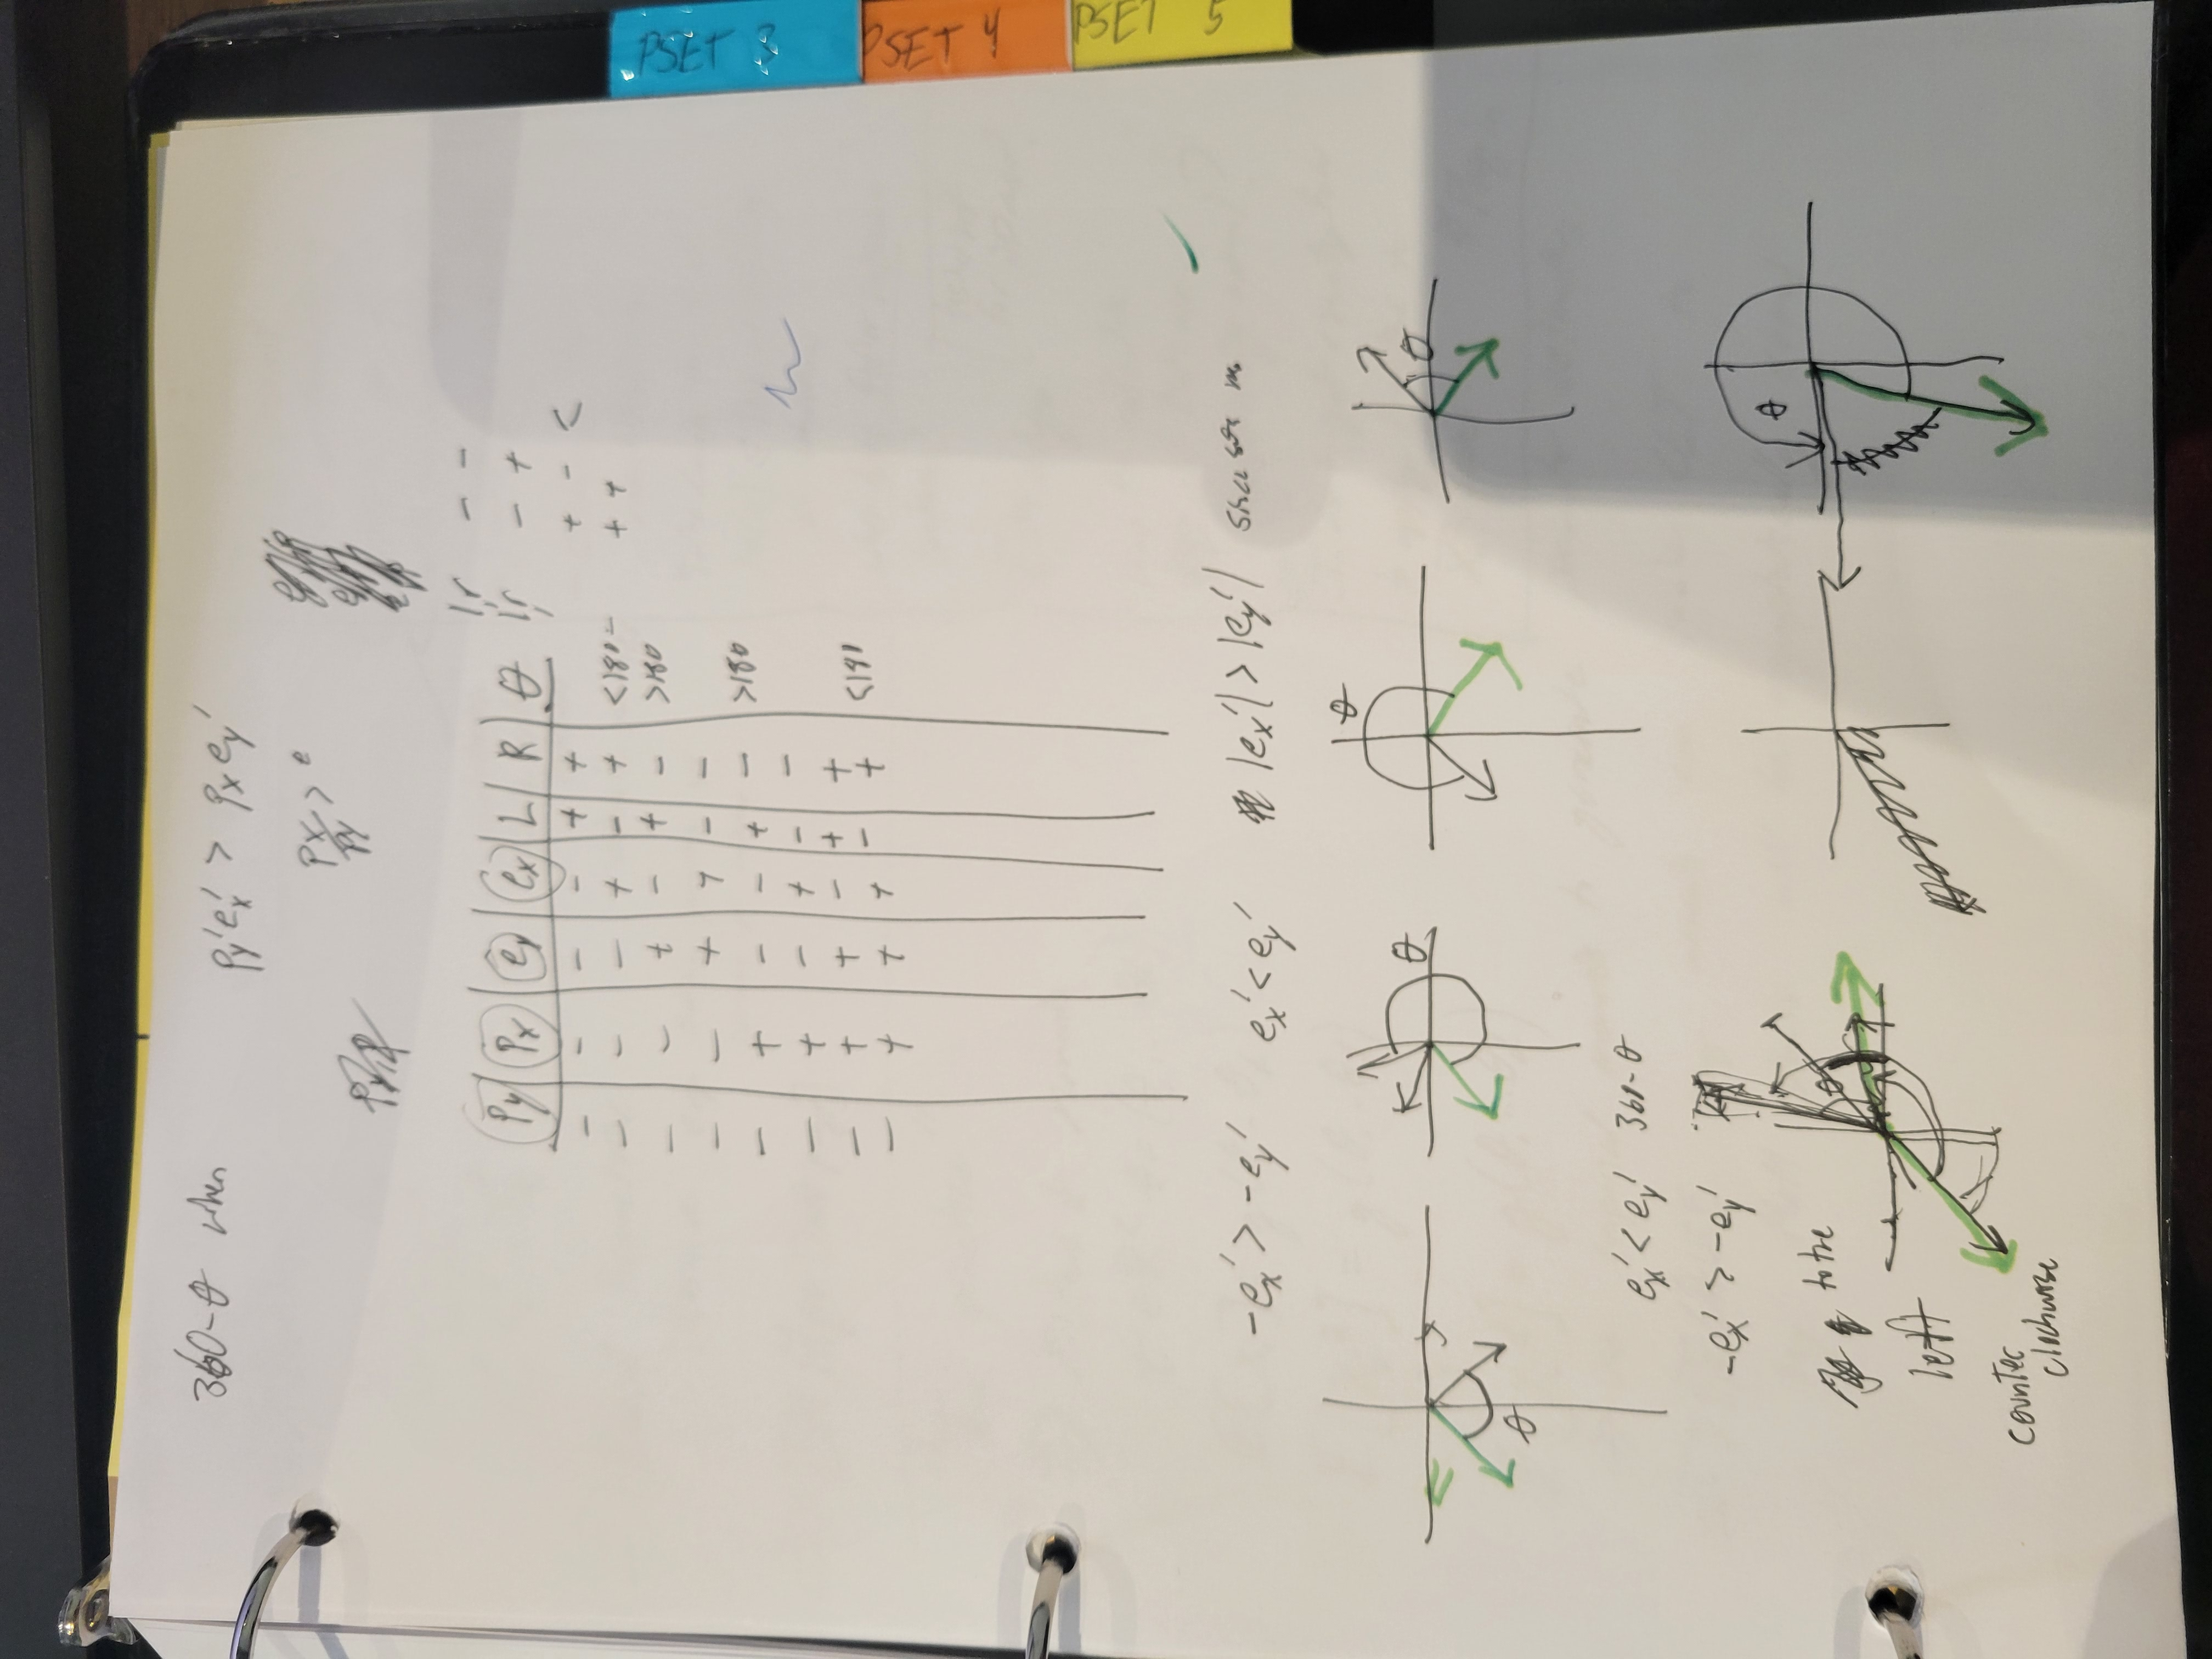
\includegraphics[width=0.9\textwidth]{Chapters/Ch1-Intro/Ch1-Sec2-GPDs-DVMP/pics/phi_math_1.jpg}       
            


Low t-data are very important for the meson exclusive physics. The GPD interpretation works only in the region -t/Q2<1. From this point of view the central detector will not only  increase the total statistics by a factor more than 2 but will add the valuable data with low t.


 However, for pi0 the only data we have from Hall A are of very limited statistics and kinematics. One of their limitations was the relatively modest variation on polarization parameter (epsilon) since the beam energies we not so far apart. 
 
 Number of final events in CLAS6 DVMP? About 100K, maybe 200K. 
 
 
 
 Dear Valery

CLAS12 acceptances and resolutions are also superior to that of CLAS6. Main differences are:
- RGK has outbending torus vs inbending CLAS6 data
- the distance between the target and the PCal has increased, the FTCal extends to lower angles, and the gap between FTCal and PCal is much smaller than between IC and EC
- proton polar angle was limited to 60 deg in the e1dvcs dataset if my memory is correct

Do you have on hands the number of exclusive pi0 events published for the CLAS6 cross-sections?
We need numbers to make the case to cook the RGK data

Well over an order of magnitude more statistics at CLAS12 compared to CLAS6


    Puzzle Origin: How is quark contribution to proton spin measured?
        Do DIS with a polarized lepton on a polarized proton. The trick is to polarize the proton target in both directions, i.e. run the experiment with the target spin up and again with target spin down. Then measure the asymmetry of the scattered leptons. The EMC collaboration did this with a polarized muon simultaneously on two separate targets with opposite-sign spin. Paper is \href{https://www-sciencedirect-com.libproxy.mit.edu/science/article/pii/0550321389900898?via\%3Dihub}{Here}. To measure the spin contribution of the gluons, you collide two proton beams, first with the spins aligned and then anti-aligned. This was done at RHIC a few years back (relative to 2020). 



